%%%%%%%%%%%%%%%%%%%%%%%%%%%%%%%%%%%%%%%%%%%%%%%%%%%%%%%%%%%%%
%% HEADER
%%%%%%%%%%%%%%%%%%%%%%%%%%%%%%%%%%%%%%%%%%%%%%%%%%%%%%%%%%%%%
\documentclass[twoside]{report}

\usepackage{preamble}

\title{
GROOVE Documentation: \\
A Developer's Manual
}

\author{
Iovka Boneva, Harmen Kastenberg, Tom Staijen, and Arend Rensink \\
University of Twente\\
Department of Computer Science\\
\{bonevai,h.kastenberg,staijen,rensink\}@cs.utwente.nl
}

\date{\today}

% inlude headers
\pagestyle{headings}

% use roman page number for preface stuff
%\pagenumbering{roman}


% -----------------------------------------------------------------------------
% macros.tex
% -----------------------------------------------------------------------------

\newcommand{\GROOVE} {{\sc groove}\xspace}
\newcommand{\LTSMIN} {{\sc LTSmin}\xspace}
\newcommand{\BLISS} {{\sc bliss}\xspace}
\newcommand{\VIATRA} {{\sc viatra2}\xspace}
\newcommand{\PINS} {{\sc pins}\xspace}
\newcommand{\NAUTY} {{\sc nauty}\xspace}

\newcommand{\Lab}{\mathsf{Lab}}
\newcommand{\Node}{\mathsf{Node}}
\newcommand{\Val}{\mathsf{Val}}
\renewcommand{\Int}{\mathsf{Int}}
\renewcommand{\Nat}{\mathsf{Nat}}
\renewcommand{\Bool}{\mathsf{Bool}}
\renewcommand{\Real}{\mathsf{Real}}
\newcommand{\String}{\mathsf{String}}
\newcommand{\Graph}{\mathsf{Graph}}
\newcommand{\X}{\mathsf{X}}

\newcommand{\nc}{\mathit{nc}}
\newcommand{\gc}{\mathit{gc}}
\newcommand{\can}{\mathit{can}}
\newcommand{\hash}{\mathit{hash}}
\newcommand{\lab}{\mathit{lab}}
\newcommand{\out}{\mathit{out}}
\newcommand{\self}{\mathit{self}}
\newcommand{\col}{\mathit{color}}
\newcommand{\ord}{\mathit{ord}}


%%%%%%%%%%%%%%%%%%%%%%%%%%%%%%%%%%%%%%%%%%%%%%%%%%%%%%%%%%%%%
%% DOCUMENT
%%%%%%%%%%%%%%%%%%%%%%%%%%%%%%%%%%%%%%%%%%%%%%%%%%%%%%%%%%%%%
\begin{document}

\maketitle

% we use the \cleardoublepage command whenever we start a new chapter in order
% to be sure that this chapter begins at the next available odd-numbered page
\cleardoublepage
\chapter*{Preface}

We are happy to present to you a document describing the fundamentals of the GROOVE Tool Set. In the coming pages we will provide the reader from a (hopefully) clear overview of the architecture of the tools within the GROOVE Tool Set.

Next to providing an overview of the structure of the tool, it is also meant as a starting point for those people just joining the GROOVE development team. We describe some basic principles that form the ground floor when writing new code for the tool, including some conventions which each developer should apply strictly.

For more information and downloads, we refer to the \GROOVE website: \url{http://groove.sourceforge.net/}

\vspace{0.2in}
\noindent
\hfill The GROOVE development team

\noindent
\hfill Enschede, The Netherlands

\tableofcontents

\cleardoublepage
% use arabic page numbering
%\pagenumbering{arabic}
% and start at 1
%\setcounter{page}{1}

\section{Introduction}

%%%% PAPER %%%%
Aspect-oriented programming (AOP) \cite{DBLP:conf/ecoop/KiczalesLMMLLI97} is a popular para{\-}digm that allows for the modular specification of cross-cutting concerns. However, aspect-oriented programs are not easy to get right and even harder to test or debug. For this reason, it is attractive to investigate formal verification for aspectual programs. For the purpose of formal verification of AOP languages and programs, it is essential to specify the semantics of such languages formally and unambiguously.\\
In this paper we present an operational semantics for Assignment Featherweight Java (AFJ), which is an extension to Featherweight Java (FJ), a minimal subset of Java. This simple language - although not suitable for industrial implementations - is often used for studying the consequences of language extensions. We study an extension of this language with \emph{around advice}, which can  --- combined with a \emph{proceed} statement -- be used to represent before and after advice.\\
\\
The specification method in this paper is graph transformations. We claim that graph transformation has two main advantages over traditional, more mathematical notations of operational semantics:
\begin{list}{$\bullet$}{}
\item Graph transformation is a formal specification technique that supports rule based specification as well as an intuitive visual representation of states and rules.
A graph transformations-based operational semantics is better comprehensible than a specification using a mathematical notation.
\item A graph transformation-based operational semantics directly provides an executable model; given a start graph representing an AFJ program and the graph transformation based operational semantics of the language, this system can be simulated resulting in a labelled transition system (LTS), sometimes better known as a state space or a meta-graph.
\end{list}

By giving the semantics in this way, the road is opened towards applying existing verification methods, such as the work we have presented in \cite{Staijen+2009}. Also, the LTS lends itself directly for model checking (see \cite{KastenbergRen2006}).\\
\\
To increase confidence in the correctness of our definitions, we show that they coincide with a formal specification of the AFJ language in a work called the Common Aspect Semantics Base (CASB) \cite{DDFL-NoE06}. The CASB is a reference model for the runtime semantics of aspect-oriented programming languages.  This work presents a structural operational semantics (SOS) for a the language at hand (AFJ with aspectual extension).\\
\\
In the next section we will explain details of Assignment Featherweight Java with around advice.
Section \ref{sec:gratra} provides a background on graph transformations and the visual notation used in this paper.
In Section \ref{sec:gr-state}, the graphs are described that represent AFJ programs with advice.
In Section \ref{sec:gr-rules} we provide a detailed description of the graph transformation based specification of chosen language. 
In Section \ref{sec:correctness} we discuss the reference semantics and formulate the notion of correctness.
Section \ref{sec:simulation} shows some example programs and shows the result of simulation.
Finally, in Section \ref{sec:relatedwork} we discuss related work, followed by our conclusions in Section \ref{sec:gr-conclusion}.


\cleardoublepage
\chapter{Background}
\chlabel{Background}


\section{The GROOVE project}

\GROOVE is an acronym of {\bf GR}aphs for {\bf O}bject {\bf O}riented {\bf VE}rification. In this project we work towards a method in which graphs are used for describing the structure of states of object-oriented programs. Such states mainly consist of objects that have been created during execution and their inter-relationships.

If each of the state of such a program is modelled by a single graph, the quesion is still how to relate (or order) all these graphs in a meaningful way. The obvious relation to chose is their temporal appearance. In other words, graphs representing subsequent states of a program should be related.

These relations between states are specified as applications of {\em graph transformation rules}. Intuitively, a graph transformation rule specifies how to make (local) changes to a certain graph. More formally, a graph transformation rule consists of a left hand side graph (\lhs) and a right hand side graph (\rhs) together with a graph morphism mapping elements of \lhs to elements of \rhs and a set of {\nac}s, being supergraphs of \lhs. It is not our intention to give an introduction to this field in this document, but rather refer to \cite{Heckel2006} which contains sufficient pointers for further reading.


\section{The GROOVE Approach}

Within the \GROOVE Tool Set the theory of graph transformation is applied on what are often called {\em simple graphs}. Simple graphs, as graphs in general, consists of a set of {\em nodes} and a set of {\em edges}. Edges, however, do not have an identity, but are identified by their {\em source node}, {\em target node}, and {\em label} instead. Therefore, edges with the same source node, target node, and label necessarily need to be equal, or stated differently, {\em parallel edges} are not allowed.

In \cite{GG-Handbook-I} the two main graph transformation approaches, namely the Single Pushout (\spo) and the Double Pushout (\dpo) approach, are explained and compared in detail. In \GROOVE we apply the \spo approach, mainly because the \dpo approach is not defined on simple graphs with partial graph morphisms. Shortly, the \spo approach unconditionally applies the graph transformation rules. If then, rule applications result in ill-formed graphs, i.e. graphs containing {\em dangling edges} for which either their source node or target node is not defined, those graphs are made well-formed again by removing the ill-formed part, i.e. by removing those dangling edges.

\section{Visualizing Transformation Rules}

Traditional graph transformation approaches specify a transformation rule by showing each component, i.e. its \lhs, \rhs, and all {\nac}s, separately. \fref{traditional-rule} is an example of such a traditional way of specifying a transformation rule. Graph morphisms are typically defined by means of the placing of the graph elements (i.e. nodes and edges).

\begin{figure}[htp]
  \centering
  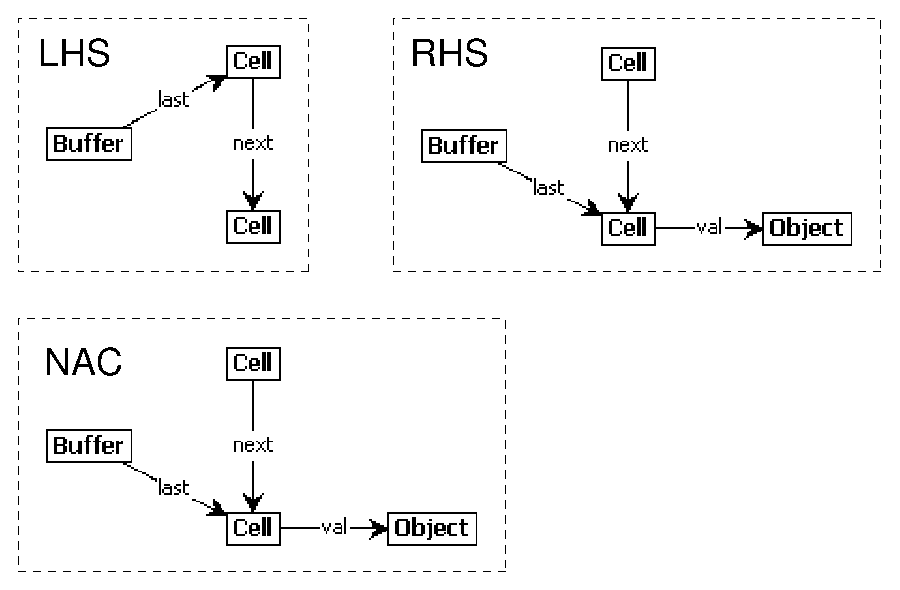
\includegraphics[scale=.75]{\figdir/traditional-rule}
  \caption{Traditional representation of a transformation rule.}
  \flabel{traditional-rule}
\end{figure}

In the GROOVE Tool Set we use a single graph representation of transformation rules. In this we depict the different roles of the graph elements by using different shapes and colours. We distinguish between four roles:

\begin{itemize}
  \item{{\em reader}: these are the nodes and edges that are only read by the rule, i.e. they are both in \lhs and \rhs. Reader nodes and edges are depicted as solid, black rectangles and arrows;}
  \item{{\em erasor}: these are the nodes and edges that are removed by the rule, i.e. they are only in \lhs. Erasor nodes and edges are represented by blue, dashed rectangles and arrows;}
  \item{{\em creator}: these are the nodes and edges that are created by the rule, i.e. they are only in \rhs. Creator nodes and edges are represented by solid, fat, green rectangles and arrows;}
  \item{{\em embargoe}: these are the nodes and edges that are forbidden for the rule to be applicable, i.e. they must not be present in the graph on which we want the rule to be applicable. Embargoe nodes and edges are represented by solid, fat, red rectangles and arrows.}
\end{itemize}

In \fref{groove-rule}, the single graph representation of the rule from \fref{traditional-rule} is shown.

\begin{figure}[htp]
  \centering
  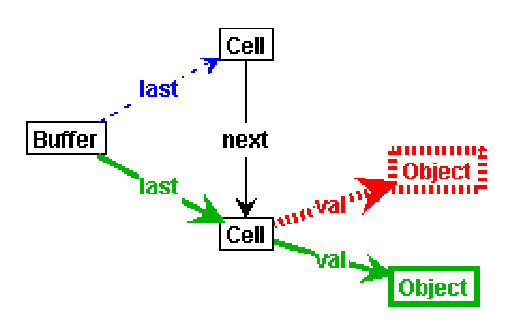
\includegraphics[scale=0.75]{\figdir/groove-rule}
  \caption{The GROOVE's single graph representation of \fref{traditional-rule}.}
  \flabel{groove-rule}
\end{figure}



\cleardoublepage
\chapter{The GROOVE Tool Set}
\chlabel{The GROOVE Tool Set}

\section{Tool Chain}

The GROOVE Tool Set basically consists of the following components:

\begin{itemize}
  \item{the simulator,}
  \item{the editor,}
  \item{the generator,}
  \item{the imager, and}
  \item{the model checker.}
\end{itemize}

\fref{tool-chain} gives an overview of how most of these tools work together, what they expect as input, and what they provide as output. The squares represent those parts of the tools that have been implemented (white background) and are planned in the future (gray background). The elipses represent the inputs and outputs for the different components.

In the following paragraphs we will shortly discuss all the implemented components, i.e. what they require as input and what they provide as output.

\begin{figure}
  \centering
  \includegraphics[scale=0.7]{\figdir/chain}
  \caption{Chain overview of the \GROOVE Tool Set.}
  \flabel{tool-chain}
\end{figure}

\section{The GROOVE Simulator}

The \GROOVE Simulator is a graphical interface enabling the user to control the \GROOVE transformation engine. It provides a direct graphical view on the state graphs, the transformation rules, and the part of the state space explored so far. Furthermore, from the Simulator the user is able to perform various actions on transformation rules, such as editing, disabling, removing, and creating new ones.

\paragraph{Input.} When starting the Simulator, it can be provided from a path to some directory containing a graph production system. Such directories should have the \texttt{.gps} `extension', otherwise the Simulator will not be able to load it succesfully. These graph production systems typically contain a (possibly empty) set of transformation rules together with a start graph named \texttt{start.gst}. When starting the Simulator from the command-line, it is possible to provide it from a different start graph, which may not be in the same directory as the transformation rules are in.

\paragraph{Output.} Apart from the visual feedback, the Simulator does not automatically provide physical output in the sense of log-files, for instance. At any point during the execution of the production system, it is possible to export the state graphs or individual rules or the transition system generated so far, to a GXL-file.


\section{The GROOVE Editor}

The GROOVE Editor provides means for specifying graphs and transformation rules. From the Editor one is able to create new or modify existing graphs and rules. It does not require any input. Its output consists of the graphs and transformation rules saved by the user.


\section{The GROOVE Generator}

The GROOVE Generator is a useful tool when users are only interested in the outcome of applying the rules of a production system to a specific graph as long as possible, without the need to look at the transformation process itself.

For example, when providing the Generator from a graph production system, it can be asked to save all the final states, i.e. the states in which no rule is applicable anymore.

\paragraph{Input.} The required input is the same as for the Simulator, i.e. a path to the directory containing a graph production system. The Generator can also be provided from a different start graph. Furthermore, the Generator has some options for directing the transformation process. These are, among others, the strategy to use for the transformation process and a file to write the results to.

\paragraph{Output.} When the Generator has finished, it should have written the required result to the specified location. Optionally, it creates a log-file containing some statistics about the transformation process.


\section{The GROOVE Imager}

With the GROOVE Imager one is able to create images from both graphs and transformation rules in various formats, such as JPG, PNG, and EPS.

\section{The GROOVE Model Checker}

Currently, the GROOVE Model Checker supports the verification of properties specified as CTL formulae over finite state graph production systems.

The Model Checker is a command-line tool which, given a graph production system generating a finite state space, first does the state space generation and subsequently asks the user for properties to be verified over this state space. The user is able to check multiple properties in sequence without the need to generate the state space over and over again.

\paragraph{Input.} The input for the Model Checker is equivalent to that of the Generator. After the transformation process, the user is asked to enter CTL formulae that have to be checked, or quit the program.

\paragraph{Output.} Currently, the Model Checker only provides output stating that a given temporal formula is satisfied by the system as specified by the graph production system or is not satisfied.

\cleardoublepage
\chapter{Tool Architecture}
\chlabel{Tool Architecture}

In this chapter we will discuss the internal structure of the \GROOVE Tool. We will explain the different Java packages all classes and interfaces are spread over.

\section{Packages}

\tblref{packages} enumerates the different packages (in alphabetical order) and gives a short description for each of them.

\begin{table}[htp]
  \centering
  \begin{tabular}{|c|p{3.5in}|}
  \hline
    {\bf Name} & {\bf Description} \\
    \hline
    \hline
    {\tt groove.algebra} & package providing the algebraic structure for attributed graphs \\
    \hline
    {\tt groove.calc} & package providing classes using graph transformations as a calculation tool \\
    \hline
    {\tt groove.graph} & package containing the basic interfaces and classes implementing graphs using different internal structures \\
    {\tt groove.graph.algebra} & package providing the necessary graph elements for attributed graphs \\
    {\tt groove.graph.aspects} & \\
    {\tt groove.graph.iso} & package providing functionality for determining isomorphism relations between graphs based on {\em graph certificates} \\
    \hline
    {\tt groove.gui} & package containing the classes implementing the graphical user interface of the \GROOVE Tool Set \\
    {\tt groove.gui.jgraph} & package containing classes that serve as an intermediate level between the \GROOVE transformation engine and the JGraph third party library used for visialization \\
    {\tt groove.gui.layout} & package providing classes to manage different graph layout algorithms \\
    \hline
    {\tt groove.gxl} & \\
    {\tt groove.gxl.types} & \\
    \hline
    {\tt groove.io} & package containing I/O classes, i.e. xml marshallers and unmarshallers \\
    \hline
    {\tt groove.lts} & \\
    {\tt groove.lts.explore} & \\
    \hline
    {\tt groove.rel} & package containing interfaces and classes featuring the use of regular expressions in transformation rules \\
    \hline
    {\tt groove.samples} & \\
    \hline
    {\tt groove.test} & package containing JUnit classes for testing the GROOVE Tool Set \\
    {\tt groove.test.graph} & subpackage containing specialized test-classes for different graph implementations \\
    \hline
    {\tt groove.trans} & package containing interfaces and classes that form the actual graph transformation engine \\
    {\tt groove.trans.view} & package providing functionality for displaying transformation rules in the typical \GROOVE single-graph representation \\
    \hline
    {\tt groove.util} & package providing small utilities used internally throughout the \GROOVE Tool Set \\
    {\tt groove.verify} & package containing interfaces and classes providing the model checking functionality of the \GROOVE Tool Set \\
    \hline
  \end{tabular}
  \caption{Overview of Java-packages within the \GROOVE Tool Set.}
  \tbllabel{packages}
\end{table}

\section{Class Hierarchies}

\subsection{Graphs}

The notion of graphs can be used at different levels. Especially in \GROOVE, we distinghuis between ordinary graphs just consisting of nodes and labeled and directed edges. On the other hand, we also use graphs to model {\em transition systems} in which the nodes are graphs themselves and edges represent rule applications. In order to make this possible, the \Graph-interface has different sub-interfaces as shown in \fref{graph-hierarchy}.

\begin{figure}
  \centering
  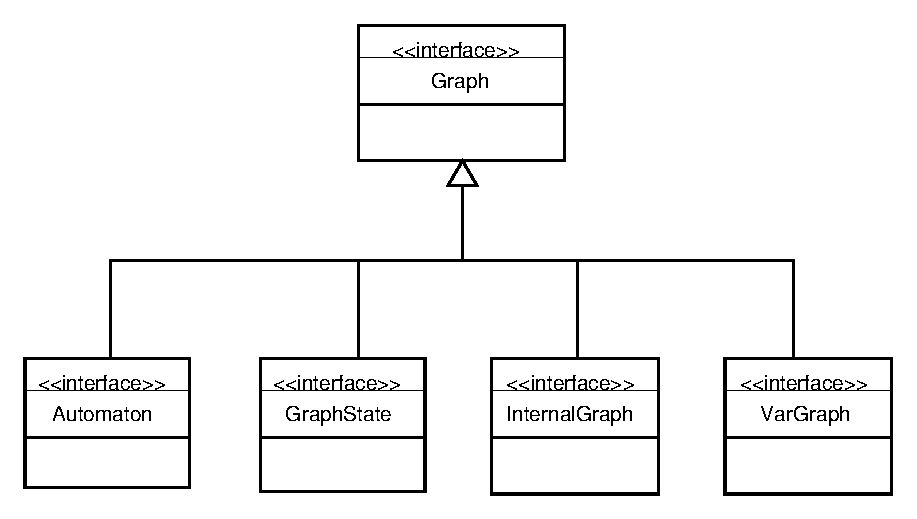
\includegraphics[scale=0.7]{\figdir/graph-hierarchy}
  \caption{The \Graph interface with different sub-interfaces.}
  \flabel{graph-hierarchy}
\end{figure}

Within the GROOVE Tool Set different implementations of graph structures are available. They mainly differ in the way they access their components. \fref{graph-hierarchy} gives an overview of the most frequently used graph implementations. For each of these we will explain the idea behind those specific implementations.

\subsection{Applied Patterns}

\subsubsection{Model View Controller}

%\cleardoublepage
%\include{license}

\cleardoublepage
\chapter{Guidelines}
\chlabel{Guidelines}


\section{Documentation}

One of the most important things in programming is good and consistent documentation. Javadoc provides a good starting point for this. We therefore require all classes, methods, and fields to be accompanied with appropriate descriptions of their intent, possibly with cross-references to other Java classes.

\section{Package Size and Dependencies}

The basic guideline for packages is to keep the number of classes within reasonable size. The exact maximum number of classes within a package is of course debatable, but this number should never exceed e.g. 100.

Concerning the dependency relations between packages we can be more clear. The basic guideline is to have only {\em one-directional} dependencies between packages.


\section{Coding Conventions}

For accessing class fields we apply the following guidelines. The general principle is that of {\em lazy initialization}. This means that whenever accessing a field \x through its \getX-method, we will first check whether \x has already been initialized or is still \nullPnt. If it is \nullPnt, we call the (protected) \computeX-method. The \computeX-method first calls the \createX-method after which it may still need to do some additional computations. The \createX-method only creates a new instance of the correct type.

Listing \ref{l:X-lazy.java} gives an overview of the things discussed above.

\codelisting{java}{X-lazy.java}{Lazy initialization.}

\subsection{Method Level}

\section{Peer Reviews}

Keeping code clear and understandable requires quite a lot of effort. In order to decentralize this process, developers can now and then schedule so called `code reviews'. Code reviews are performed on pieces of code written by other developers. When things are unclear this should be indicated by what we call {\em personal tags}.

\subsection{Personal Tags}

In order to be able to keep track of code being reviewed, individual tags have been introduced for each developer. That is, whenever you review a class or method and want to add some comments, you should include your personal tag (your first name in capital letters) followed by the actual comment. The idea is then that every now and then, developers should take a quick look at all the comments and see whether some comments require some discussion or simple actions to be taken. The use of personal tags is shown in Listing \ref{l:X.java}.

\codelisting{java}{X.java}{Personal tags.}


\cleardoublepage
\chapter{Data Structures and Algorithms}
\chlabel{Data Structures and Algorithms}

In this chapter we give a description to some of the most complex
algorithms and data structures in the \GROOVE implementation. This should
help the developer to have a relatively high-level view on \GROOVE. This
description is to be considered together with the {\em javadoc} that gives
a detailed explanations on the classes / methods, that we do not reproduce
here.

\section{Storage of Graphs}
\stlabel{storage of graphs}

The tool \GROOVE manipulates a labelled transition system that may contain
a very big number of graphs as states. Space is a critical resource for the
tool, and efficient storage of graphs is essential.

There are two essential mechanisms in \GROOVE that are related to efficient
graph storage, while trying to keep an optimal time performance:
\begin{itemize}
\item a {\em delta graph} is a representation of a graph expressed by the
  changes that one should operate on some {\em basis graph} in order to
  obtain it. {\em Changes} are added and removed elements (nodes or edges).
  Delta graphs are very useful as in a labelled transition system most of
  the new graphs are generated by graph transformation, thus share lots of
  common structure with other graphs. This is the format in which graphs
  are represented in run-time;
\item a {\em graph cache} is a representation of a graph as a set of nodes
  and a set of edges with additional information in order to make graph
  processing easier. If the JVM runs out of memory, the garbage collector
  is authorised to remove cache graphs. If some computations with a graph
  are involved, then the cache is recomputed again.
\end{itemize}

On \fref{graphs} we depict the class hierarchy relative to the
representation of graphs and delta graphs in \GROOVE. On \fref{elements} is
represented partially the class hierarchy relative to graph elements
(nodes, edges). Finally, \fref{caches} gives a portion of the class
hierarchy related to graph caches. For further details, we refer to the
{\em javadoc}.
\begin{figure}[ht]
  \centering
  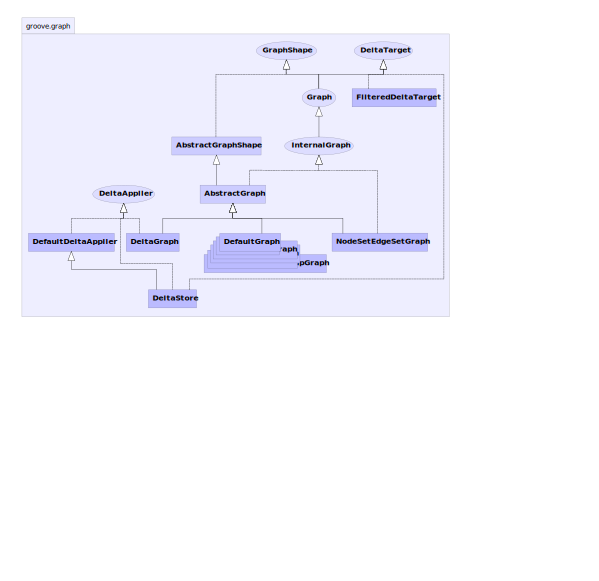
\includegraphics{fig/graphs}
  \caption{Graph related class hierarchy.}
  \flabel{graphs}
\end{figure}

\begin{figure}[ht]
  \centering
  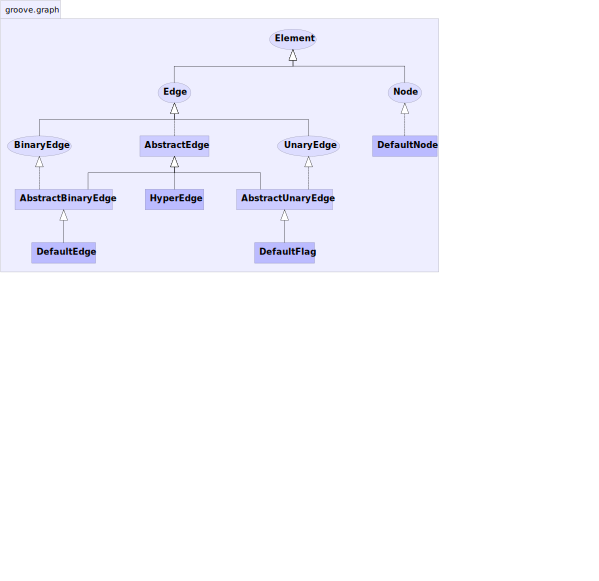
\includegraphics{fig/elements}
  \caption{Part of the class hierarchy relative to graph elements.}
  \flabel{elements}
\end{figure}

\begin{figure}[ht]
  \centering
  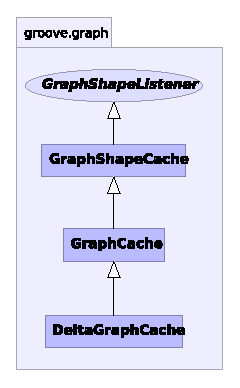
\includegraphics{fig/caches}
  \caption{Part of the class hierarchy relative to graph cache.}
  \flabel{caches}
\end{figure}

\paragraph{Delta Graph}
A {\em delta graph} is essentially a basis graph together with a set of
added elements and a set of removed elements (nodes or edges). For storage
optimisation, added and removed elements are stored into a single array,
called {\em delta array}. The basis graph can also be a delta graph.  Thus,
we can have a sequence of delta graphs, each of which is used as a basis of
the next one. Very long such sequences may result in a big loss of time
efficiency, as most of the manipulations on a graph require a node-set
edge-set based representation, which should be recomputed. Therefore, the
length of such sequences is limited to at most {\tt
  graph.DeltaGraphCache.FREEZE\_DEPTH}, currently set to $8$.
% TODO : what is a frozen delta graph ?
% TODO : make sure that it is indeed the limit

\paragraph{Graph Cache}
A graph cache is a representation of a graph that contains explicitly the
sets of nodes and edges of the graph, as well as adjacency map associating
with each node its adjacent edges, and edge label map, associating with
each label the edges wearing this label. This redundant representation
facilitates computations on a graph. 

An object of type {\tt graph.AbstractGraphShape} contains a reference to a
{\tt graph.GraphShapeCache} (in the form of a {\tt
  java.lang.ref.Reference<GraphShapeCache>} object), and it supports a {\tt
  clearCache()} operation that allows to notify the garbage collector that
the cache object can be collected in case there is a need of additional
memory.

\section{Labelled Transition System}

Remind that the \GROOVE Simulator and Generator allow to (partially)
construct the labelled transition system corresponding to some graph
grammar. Such a LTS is of the form $\mathcal S = (S, T, s_0, F)$. States in
$S$ are graphs and transitions in $T$ are of the form $(G, (P,m), H)$,
where the graphs $G,H$ are states of the labelled transition system and the
label $(P,m)$ consists of a graph production $P$ and a matching $m: L \to
G$ (with $P = (L, R)$).

The functionality of Groove related to computing and storing a Labelled
Transition System (LTS) is implemented into two packages.
\begin{itemize}
\item \texttt{lts} package for construction and storage of a labelled transition system,
\item \texttt{trans} package for computing transformations.
\end{itemize}
In what follows we describe these implementations. We start with a general
description, and then give details on the implementations. We omit the {\tt
  groove} prefix in class names (i.e. we write {\tt lts.GTS} instead of
{\tt groove.lts.GTS}).

\subsection{Interface for a Labelled Transition System}
A LTS is a graph-like structure. The interface {\tt graph.GraphShape}
defines basic graph functionality, such as adding, removing and retrieving
nodes and edges and sets of nodes and edges, etc. The interface {\tt
  lts.LTS} (\fref{lts-interface}) extends the interface {\tt
  graph.GraphShape} with the notion of start and final states and with the
method

\smallskip\noindent%
{\tt boolean isOpen(State state);}

\noindent
A state of a LTS is considered {\em open} if not all outgoing transitions have
not been explored.

\begin{figure}[ht]
  \centering
  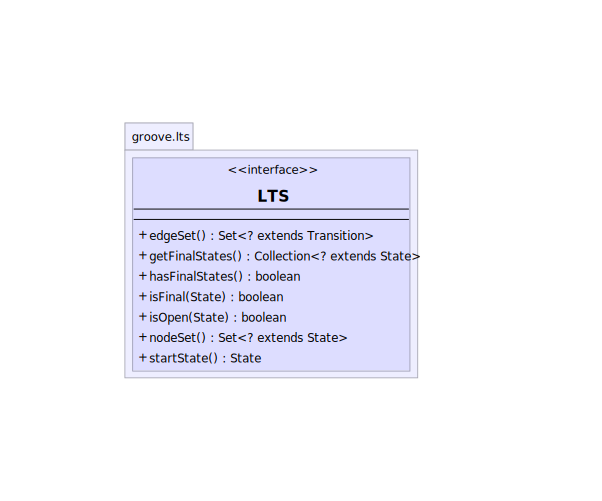
\includegraphics[scale=0.8]{fig/LTS}
  \caption{The interface {\tt lts.LTS}.}
  \flabel{lts-interface}
\end{figure}


\paragraph{States and Transitions of a Labelled Transition System}

The {\tt lts} package provides the hierarchy of states and
transitions of an LTS depicted on \fref{states and transitions}.

\begin{figure}[ht]
  \centering
  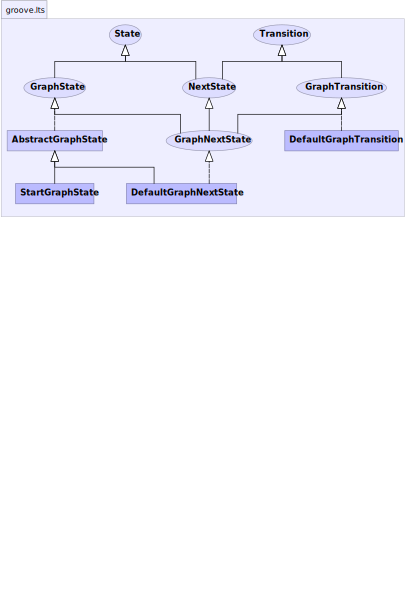
\includegraphics{fig/states-and-transitions}
  \caption{States and transitions class hierarchy for a LTS.}
  \flabel{states and transitions}
\end{figure}

The interface {\tt lts.NextState} combines a state and a transition. It is
intended to represent a state together with one of its incoming
transitions. The interface {\tt lts.GraphState}, {\tt lts.GraphTransition}
and {\tt lts.GraphNextState} specialise a state, a transition and a ``next
state'' for labelled transition systems which states are graphs and which
transitions represent direct derivations. The classes {\tt
  lts.DefaultGraphTransition}, {\tt lts.DefaultGraphNextState} and {\tt
  lts.StartGraphState} are the implementations of these interfaces. On
\fref{graphstate} we present in more detail the functionality provided by
the interface {\tt lts.GraphState}. As one can see from this figure, a {\tt
  lts.GraphState} knows its outgoing transitions. The {\tt setClosed()}
method closes the state, forbidding to add more outgoing transitions to it.

\begin{figure}[ht]
  \centering
  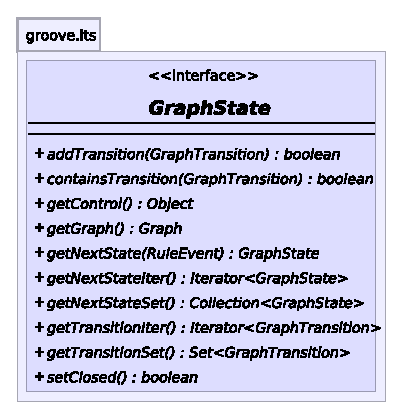
\includegraphics{fig/GraphState}
  \caption{Partial description of the interface {\tt lts.GraphState}.}
  \flabel{graphstate}
\end{figure}

\subsection{Storing a Labelled Transition System}

A labelled transition system is stored in an object of class {\tt lts.GTS}
(for Graph Transition System, i.e. transition system which states are
graphs), which implements {\tt lts.LTS}.

Let us first give an intuitive explanation of the way a LTS is stored.
Given an LTS $\mathcal S = (S, T, s_0)$, a {\em spanning tree} of $\mathcal
S$ is a tree whose set of nodes is $S$, has $s_0$ as a root, and whose
arrows are transitions in $T$ (see \fref{spanning tree} for an example of a
spanning tree). That is, a spanning tree contains all nodes of a LTS, but
not all transitions. However, if for any node we have sufficient
information allowing to reconstruct its outgoing transitions, then we can
easily reconstruct the whole LTS from its spanning tree. Storing a LTS as
one of its spanning trees allows to save space if we can store the missing
transitions in an efficient way. Now, a spanning tree can be completely
defined by its root and its set of nodes, if any node contains also its
unique (in the spanning tree) incoming arrow. This possibility is offered
by the interface {\tt lts.GraphNextState}.  We will see in the next section
how the possibility of efficient storage of an LTS by its spanning tree is
explored during the construction of an LTS.

\begin{figure}[ht]
  \centering
  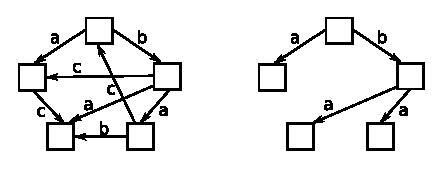
\includegraphics{fig/spanning-tree}
  \caption{A labelled transition system on the left and one of its spanning trees on the right.}
  \flabel{spanning tree}
\end{figure}

% \paragraph{Efficient Storage of Transitions in an LTS}
% As we mentioned previously, transitions of a GTS are stored as outgoing
% transitions by the states of the GTS. Therefore, it is not necessary to
% store the source state of a transition. The interface {\tt
%   lts.GraphOutTransition} describes transitions that do not know their
% source state. Its implementation {\tt lts.DefaultGraphOutTransition} thus
% defines a transition as a {\tt trans.RuleEvent} and a {\tt
%   lts.TargetState}. A {\tt trans.RuleEvent} is essentially a graph
% production and a host graph together with the image of the anchor of the
% left-hand side of the rule into the host graph. 

% \paragraph{Efficient Storage of States in an LTS}
% As described in \stref{storage of graphs}, several techniques are employed
% for efficient storage of graphs. Further optimisations can be done when
% graphs are the states of a LTS. A {\tt lts.GTS} stores its set of states as
% a set of objects of type {\tt lts.DerivedGraphState} (except for the start
% state).  As shown on \fref{states and transitions}, a {\tt
%   lts.DerivedGraphState} extends a {\tt graph.DeltaGraph}. Remind that a
% {\tt graph.DeltaGraph} stores a basis graph as well as an array of modified
% -- added and removed -- elements.  A {\tt lts.DerivedGraphState} contains
% information on its predecessor state in the spanning tree of the LTS and
% the corresponding incoming transition. The predecessor state is the basis
% graph. This transition contains the rule and the matching into the basis
% graph, thus removed elements can be deduced from it. Therefore, the delta
% array of a {\tt lts.DerivedGraphState} stores only the elements added to
% basis graph while performing the transition. These elements are also called
% {\em co-anchor image}: the image of the elements of the right-hand
% side of the rule that are new (w.r.t. the left-hand side).

\subsection{Constructing a Labelled Transition System}

The construction of a LTS is always done according to some exploration
strategy. In practise, the LTS corresponding to some graph grammar is often
infinite. Therefore, the strategy defines how to generate a portion of it
(e.g. depth-first, breadth-first). The strategy interface is given on
\fref{ExploreStrategy}.

\begin{figure}[ht]
  \centering
  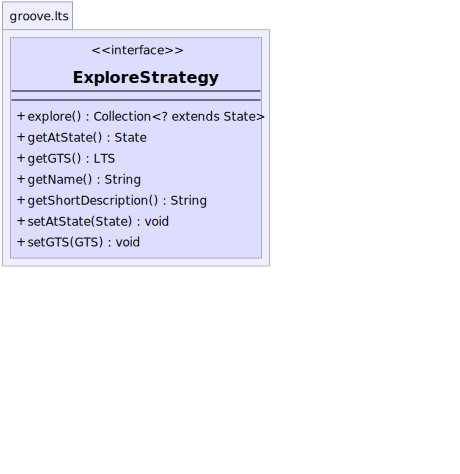
\includegraphics[scale=0.8]{fig/ExploreStrategy}
  \caption{The {\tt lts.ExploreStrategy} interface.}
  \flabel{ExploreStrategy}
\end{figure}

It allows to set the exploration at a given state ({\tt setAtState}) and to
make an exploration. For a list of the implemented strategies the reader is
invited to consult the {\em javadoc}.

The class {\tt lts.StateGenerator} that provides basic functionality for
generating new states in of a {\tt lts.GTS}, and is used as an interface by
the strategies. On \fref{StateGenerator} is depicted a partial view of the
functionality provided by this class.

\begin{figure}[ht]
  \centering
  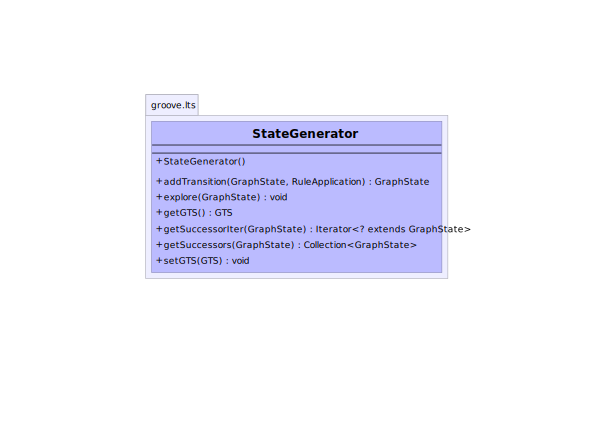
\includegraphics{fig/StateGenerator}
  \caption{Partial description of the class {\tt lts.StateGenerator}.}
  \flabel{StateGenerator}
\end{figure}

The method {\tt addTransition} adds a new transition to the associated GTS
(here a GTS) for the given source node and a {\tt trans.RuleApplication}.
The method {\tt explore} adds all (not already present) transitions to the
given state. Finally, the class gives to possibility to retrieve, or
iterate over, the successor states of a given state. 

% TODO
% We would like to describe here briefly different optimisation methods used
% while constructing the LTS.



% One can see that this class gives the possibility to compute the target
% state for some rule application, to add a transition to a LTS, or compute
% or iterate over all (already computed) successors of a given state. The
% protected method {\tt getConfluentTarget(RuleApplication)} is used for
% computing a successors state. It tries to derive the successor state
% walking around three sides of a confluent diamond instead of computing the
% state directly. When it is not possible, a {\tt lts.StateGenerator} uses a
% so called {\tt trans.Deriver} for performing the actual transformation.

% We give here only a brief description of derivers. More information can be
% find in the {\em javadoc}.

% On \fref{graph transitions} we show some hierarchies of classes used for
% representing a rule application.

% \begin{figure}[ht]
%   \centering
%   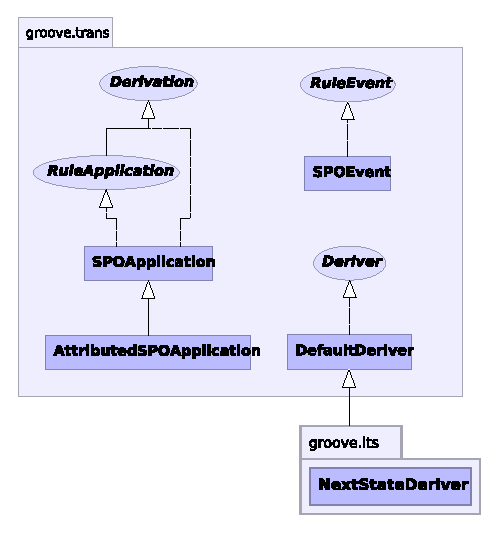
\includegraphics{fig/graph-transitions}
%   \caption{Hierarchy of classes for rule application.}
%   \flabel{graph transitions}
% \end{figure}

% Relative to the construction of the labelled transition system is the class
% {\tt lts.NextStateDeriver}. This is an implementation of a {\tt
%   trans.Deriver} that guarantees that newly generated graphs will be of
% type {\tt lts.DefaultNextState}. These is the run-time type of states of a
% {\tt lts.GTS}. Thus, a {\tt lts.StateGenerator} uses a {\tt
%   lts.NextStateDeriver} for computing graph derivations.




\addcontentsline{toc}{chapter}{Acknowledgments}
\chapter*{Acknowledgements}

UML diagrams in the present document are generated with the help of the
yDoc tool, by yWorks \url{http://www.yworks.com/en/products_ydoc.htm}.

\newpage
% Bibliography with BibTeX
% ========================
\bibliographystyle{abbrv}
\bibliography{references}

\end{document}
